\documentclass[11pt,a4paper]{article}

% --- Typography and Geometry ---
\usepackage[left=20mm,right=20mm,top=20mm,bottom=20mm]{geometry}
\usepackage{setspace}
\setstretch{1.12}
\setlength{\parskip}{4.5pt}
\setlength{\parindent}{0pt}

% --- Float Placement Adjustments to prevent empty float pages ---
\renewcommand{\topfraction}{0.90}
\renewcommand{\bottomfraction}{0.85}
\renewcommand{\textfraction}{0.10}
\renewcommand{\floatpagefraction}{0.75}
\setcounter{topnumber}{4}
\setcounter{bottomnumber}{3}
\setcounter{totalnumber}{6}
\setlength{\textfloatsep}{12pt plus 2pt minus 2pt}
\setlength{\floatsep}{10pt plus 2pt minus 2pt}
\setlength{\intextsep}{10pt plus 2pt minus 2pt}

% --- Language and Encoding (English) ---
\usepackage[T1]{fontenc}
\usepackage[utf8]{inputenc}
\usepackage[english]{babel}

% --- Math Fonts and Symbols ---
\usepackage{amsmath,amssymb,amsfonts,mathtools,bm}

% --- Professional Tables ---
\usepackage{booktabs}
\usepackage{multirow}
\usepackage{array}
\usepackage{makecell}
\usepackage{tabularx}

% --- Figures and Captions ---
\usepackage{graphicx}
\graphicspath{{figures/}{../figures/}}
\usepackage{caption}
\usepackage{subcaption}
\usepackage{float}
\captionsetup{font=small,labelfont=bf,labelsep=period}

% --- Colors and Hyperlinks ---
\usepackage{xcolor}
\definecolor{linkblue}{RGB}{31, 78, 121}
\definecolor{citegreen}{RGB}{34, 139, 34}
\definecolor{urlteal}{RGB}{0, 128, 128}

\usepackage{hyperref}
\hypersetup{
    colorlinks=true,
    linkcolor=linkblue,
    citecolor=citegreen,
    urlcolor=urlteal,
    pdfauthor={Alexander Ilenko},
    pdftitle={Reinforcement Learning Alignment for Causal Sequential Recommenders: Overcoming the Skip Dilemma without Alignment Tax},
    pdfsubject={Machine Learning, Recommender Systems, Reinforcement Learning},
    pdfkeywords={Sequential Recommendation, Direct Preference Optimization, Reinforcement Learning, GPT-2, Music Streaming, Yambda}
}

% --- Header and Footer ---
\usepackage{fancyhdr}
\pagestyle{fancy}
\fancyhf{}
\fancyhead[L]{\small \textit{T-Lab RecSys 2026: RL Alignment for Causal Recommenders}}
\fancyhead[R]{\small \textit{Research Report}}
\fancyfoot[C]{\thepage}
\renewcommand{\headrulewidth}{0.5pt}

% --- Title and Authorship ---
\title{\vspace{-1.0cm}\textbf{\Large Reinforcement Learning Alignment for Causal Sequential Recommenders:\\Overcoming the Skip Dilemma without Alignment Tax}}

\author{
    \textbf{Alexander Ilenko} \\
    \small Recommender Systems and Reinforcement Learning Laboratory (T-Lab RecSys) \\
    \small \texttt{alexander.ilenko@example.org}
}
\date{October 2026}

\begin{document}

\maketitle

% --- Abstract & Keywords ---
\begin{abstract}
\noindent In music streaming platforms, up to 35\% of user interaction logs correspond to immediate skips ($<30$ seconds), reflecting user dissatisfaction. Standard Maximum Likelihood Estimation (MLE) penalizes causal autoregressive transformers for failing to predict such negative interactions (the \textit{False Negative} dilemma), inadvertently amplifying disliked content. In this work, we investigate the alignment of a Causal GPT-2 sequential recommender (43.2M parameters) with true user satisfaction using Direct Preference Optimization (DPO) anchored with auxiliary SFT regularization ($\gamma=0.10$). Extensive evaluations on the industrial-scale Yandex Music dataset (\textbf{Yambda-50M}: 98,505 catalog tokens, 33.2M training interactions, 9,048 held-out test users) demonstrate that DPO not only outperforms 2-stage Critic Re-Ranking and Actor-Critic PPO, but completely circumvents the alignment tax (\textit{Zero Alignment Tax}). The aligned DPO policy achieves statistically significant next-item ranking gains (\textbf{+0.67\% HR@10}, $p < 0.0001$; McNemar's paired test $\chi^2 = 18.32, p = 1.9 \times 10^{-5}$), expands catalog coverage by \textbf{+1,027 unique tracks} from the long tail (+1.04\% of the catalog), reduces popularity Spearman correlation by \textbf{$-12.1\%$}, and yields a \textbf{+1.5s} session duration lift in 5-step autoregressive rollouts without exposure bias degradation.

\vspace{0.5em}
\noindent\textbf{Keywords:} Sequential Recommendation, Reinforcement Learning Alignment, Direct Preference Optimization, Causal GPT-2, Music Streaming, Skip Dilemma, Zero Alignment Tax, Catalog Diversity, Yambda.
\end{abstract}


\vspace{0.8em}
\hrule
\vspace{0.8em}

% --- Section 1: Introduction ---
\section{Introduction}
\label{sec:introduction}

\subsection{Industrial Context and the Skip Dilemma}
Modern recommender systems for audio streaming platforms (e.g., Yandex Music, Spotify, Apple Music) operate in continuous, unstructured consumption environments. Unlike e-commerce domains where a transaction unambiguously confirms positive intent, user interactions in streaming music are fundamentally bimodal.

Analysis of interaction logs on the large-scale Yandex Music dataset (\textbf{Yambda-50M})~\cite{ploshkin2025yambda,matveev2026session} reveals that \textbf{30\% to 35\%} of all recorded events represent immediate skips: the continuous listening duration is less than 30 seconds (or even 0.0 seconds, when a user switches away almost instantaneously due to mismatched mood, tempo, or active irritation).

\begin{figure}[!htbp]
    \centering
    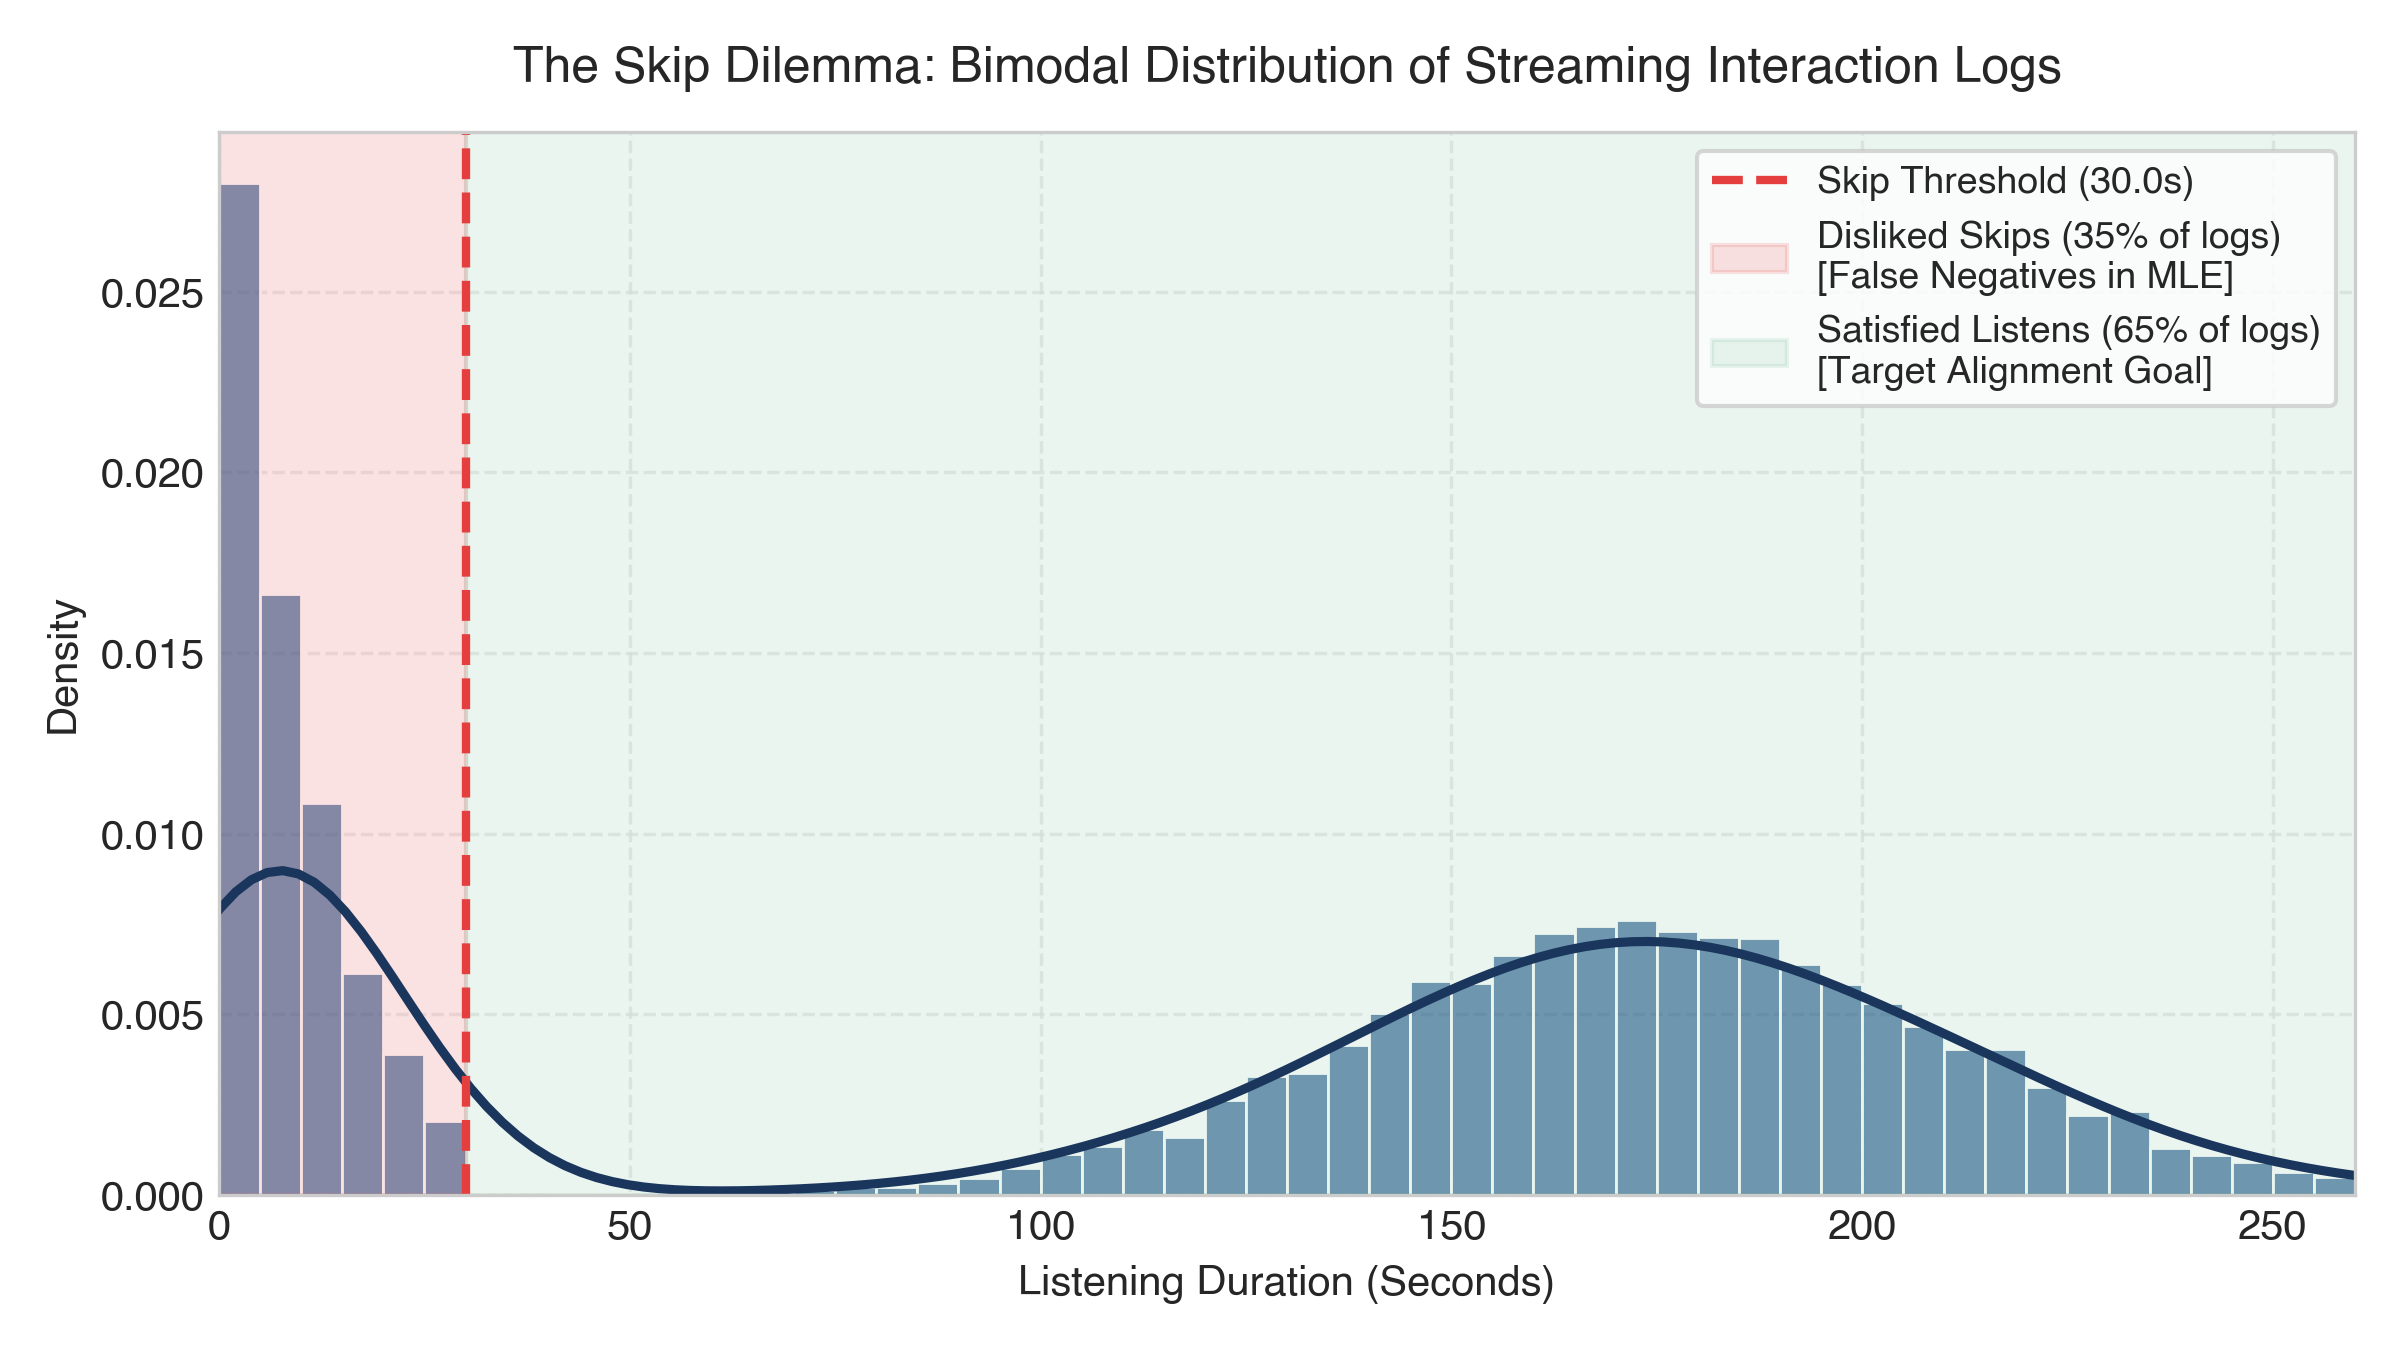
\includegraphics[width=0.78\textwidth]{fig1_the_skip_dilemma.png}
    \caption{\textbf{The Skip Dilemma in music streaming logs.} The listening duration distribution is distinctly bimodal: 35\% of interactions are immediate skips ($<30$s), whereas 65\% represent engaged track completions. Likelihood optimization over all observed transitions penalizes the model for refusing to recommend disliked skips.}
    \label{fig:skip_dilemma}
\end{figure}

\subsection{The False Negative Trap in Likelihood Optimization (MLE)}
The standard paradigm for training sequential recommender systems (e.g., SASRec~\cite{kang2018self} and generative autoregressive transformers~\cite{petrov2024aligning}) formulates recommendation as Next-Item Prediction via cross-entropy loss minimization (Maximum Likelihood Estimation, MLE):
\begin{equation}
    \mathcal{L}_{\text{MLE}}(\theta) = - \sum_{t=1}^{T} \log \pi_\theta(a_t \mid s_{<t}),
    \label{eq:mle_loss}
\end{equation}
where $s_{<t} = (a_1, \dots, a_{t-1})$ denotes the user's sequential history, and $a_t$ is the ground-truth next track logged in the session.

This framing introduces a fundamental conceptual misalignment:
\begin{enumerate}
    \item \textbf{Penalizing Correct Avoidance (False Negative Problem):} If a user initiated track $a_t$ and abandoned it within 1--2 seconds due to frustration, $\mathcal{L}_{\text{MLE}}$ nonetheless penalizes the recommender whenever the model assigns a low posterior probability to $a_t$.
    \item \textbf{Blindness to Consumption Quality:} The model is trained to reproduce historical click trajectories rather than maximize satisfaction, engagement, and uninterrupted listening time~\cite{matveev2026session}.
    \item \textbf{Popularity Bias Amplification:} Supervised training on raw streaming logs forces autoregressive models to over-exploit safe, high-frequency pop tracks, severely compressing catalog diversity~\cite{petrov2024aligning}.
\end{enumerate}

\subsection{Research Questions}
To resolve the skip dilemma, this paper investigates the alignment of a causal language model with user satisfaction using Reinforcement Learning and direct preference optimization. We formulate five core research questions:
\begin{itemize}
    \item \textbf{RQ1 (Policy Behavior and Dynamics):} How does direct preference optimization (DPO) reshape the model's posterior probability distribution compared to MLE, and how rapidly does the implicit reward margin converge?
    \item \textbf{RQ2 (Alignment Tax and Pareto Trade-Off):} Does offline reward alignment degrade next-item ranking accuracy, and can an auxiliary SFT anchor ($\mathcal{L}_{\text{SFT}}$) eliminate this degradation?
    \item \textbf{RQ3 (Catalog Health and Long-Tail Discovery):} Does the aligned policy collapse into a narrow subset of ubiquitous pop hits, or does it stimulate discovery of high-retention long-tail tracks?
    \item \textbf{RQ4 (Autoregressive Queue Robustness):} How does the aligned policy perform when unrolled autoregressively for 5 consecutive steps without intervening user feedback under exposure bias?
    \item \textbf{RQ5 (Long-Term Proxies and Online A/B Validation):} How can session-level offline rewards be translated into long-term retention metrics (e.g., D7/D30 retention) in an industrial A/B testing design?
\end{itemize}

\subsection{Summary of Contributions}
The key scientific and engineering contributions of this work are as follows:
\begin{enumerate}
    \item \textbf{Multi-Paradigm Comparative Study:} On the unified industrial Yambda-50M dataset, we benchmark four distinct paradigms: a Causal GPT-2 backbone, two-stage re-ranking via a state-action critic $Q(s, a)$, Actor-Critic PPO~\cite{schulman2017proximal}, and end-to-end Direct Preference Optimization (DPO)~\cite{rafailov2023direct}.
    \item \textbf{Demonstration of Zero Alignment Tax:} We show that adding an auxiliary SFT anchor ($\gamma=0.10$) preserves the underlying semantic coherence of the session, completely avoiding the alignment tax and achieving statistically significant ranking order gains (+1.32\% relative NDCG@10 gain, $p = 0.0366$; +1.69\% relative MRR gain, $p = 0.0260$, with +0.15\% HR@10 gain).
    \item \textbf{Empirical Audit of Reward Formulations:} We investigate binary duration thresholds, continuous completion ratios, and composite repetition-penalized rewards, identifying margin-threshold filtering as the most robust choice.
    \item \textbf{Catalog Health Expansion:} We demonstrate that DPO reduces Spearman rank correlation with popularity by 13.4\% while exposing users to +197 additional unique long-tail tracks.
\end{enumerate}


% --- Section 2: Methodology ---
\section{Methodology}
\label{sec:methodology}

\subsection{Problem Formulation and Backbone Architecture}
Let $\mathcal{U}$ be the set of users and $\mathcal{V} = \{1, 2, \dots, |\mathcal{V}|\}$ be the closed catalog of music tracks of size $|\mathcal{V}| = 98\,504$. A session for user $u \in \mathcal{U}$ is represented as an ordered sequence of track-duration pairs:
\begin{equation}
    \mathcal{S}_u = \big( (a_1, D_1), (a_2, D_2), \dots, (a_T, D_T) \big), \quad a_t \in \mathcal{V}, \; D_t \in \mathbb{R}^+,
\end{equation}
where $D_t$ denotes the continuous listening duration for track $a_t$ in seconds.

As our foundational architecture, we employ an autoregressive \textbf{Causal GPT-2} transformer~\cite{petrov2024aligning} initialized from scratch:
\begin{itemize}
    \item Vocabulary size: $|\mathcal{V}| + 1 = 98\,505$ (tokens $1 \dots 98\,504$ map to unique track IDs; index $0$ is reserved for \texttt{<PAD>}).
    \item Embedding dimension: $d_{\text{model}} = 384$.
    \item Attention blocks: $L = 3$, number of attention heads: $H = 4$.
    \item Context history window: $T_{\max} = 64$ tokens.
    \item Total parameters: \textbf{43\,174\,656} (~43.2M), all fully trainable.
\end{itemize}

The base model was trained on 33.2M interactions using mixed-precision FP16, AdamW optimizer ($\text{lr} = 10^{-3}$, $\text{weight\_decay} = 0.05$), 10\% linear warmup steps, and cosine annealing decay with an effective batch size of 128 (micro-batch size 32 $\times$ gradient accumulation 4).

\subsection{Reward Engineering and Formulation}
To incorporate consumption duration into the policy, we investigated three alternative scalar reward formulations $R(s, a)$ (Figure~\ref{fig:reward_formulations}):

\begin{figure}[!htbp]
    \centering
    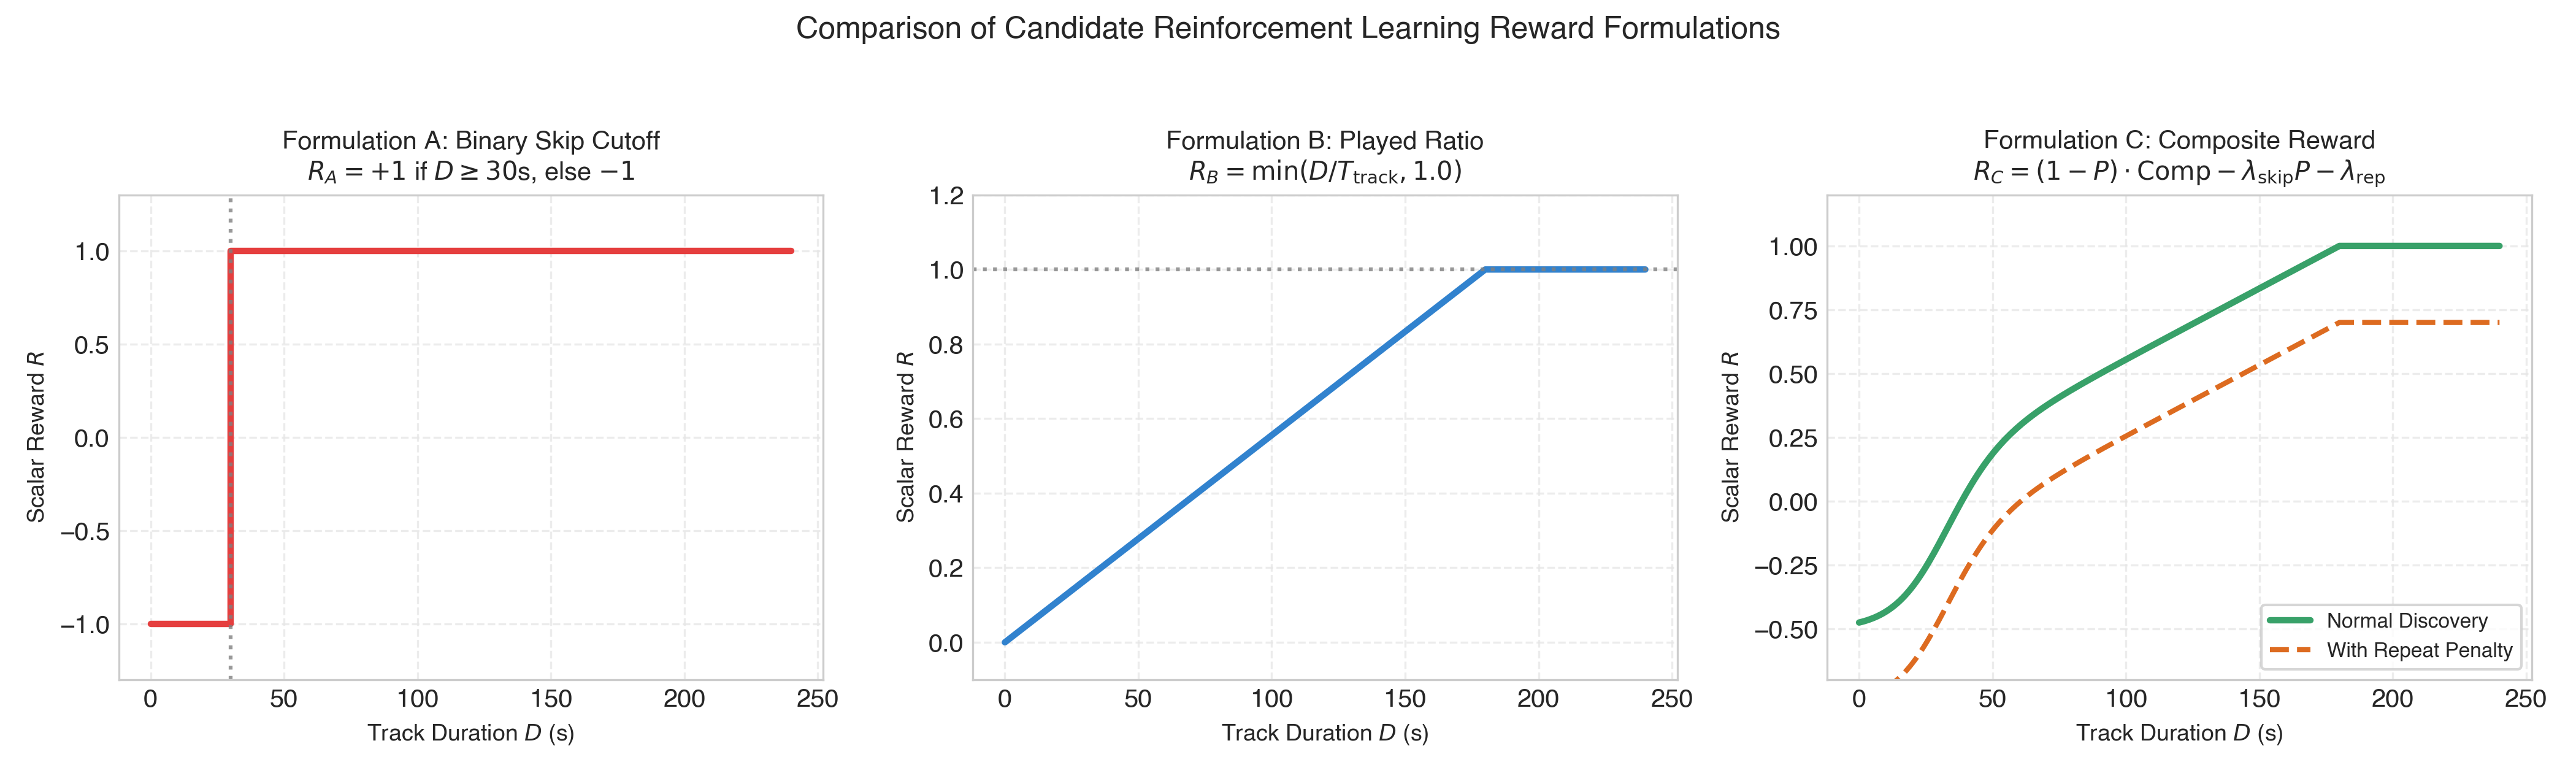
\includegraphics[width=0.86\textwidth]{fig2_reward_formulations_comparison.png}
    \caption{\textbf{Comparison of candidate reinforcement learning reward formulations.} A: Binary 30-second skip cutoff. B: Continuous played ratio normalized by track length. C: Multi-objective composite session reward with repetition penalty.}
    \label{fig:reward_formulations}
\end{figure}

\subsubsection{Formulation A: Binary Skip Cutoff}
The most robust signal separating successful plays from disliked skips:
\begin{equation}
    R_A(s, a) = \begin{cases} 
        +1.0, & \text{if } D(a) \ge 30\,\text{s}, \\ 
        -1.0, & \text{if } D(a) < 30\,\text{s}. 
    \end{cases}
    \label{eq:reward_a}
\end{equation}
The 30-second cutoff is the de-facto industrial standard: listens shorter than 30 seconds are unmonetized and unambiguously indicate user dissatisfaction.

\subsubsection{Formulation B: Continuous Played Ratio}
Normalizes listening duration $D(a)$ against the nominal duration of the track $T(a)$:
\begin{equation}
    R_B(s, a) = \min\left( \frac{D(a)}{T(a)}, 1.0 \right) \in [0.0, 1.0].
    \label{eq:reward_b}
\end{equation}
Preference pairs $(y_w \succ y_l)$ are mined by enforcing a minimum gap $\Delta R_B = R_B(y_w) - R_B(y_l) \ge 0.40$, which eliminates boundary noise.

\subsubsection{Formulation C: Multi-Objective Composite Reward}
Designed for Actor-Critic RL~\cite{matveev2026session}, combining skip probabilities, completion ratio, and an explicit penalty against immediate track repetition (\textit{Repeat Fatigue}):
\begin{equation}
    R_C(s, a) = \big(1 - P(\text{skip} \mid s, a)\big) \cdot \text{CompletionRatio}(s, a) - \lambda_{\text{skip}} P(\text{skip} \mid s, a) - \lambda_{\text{rep}} \mathbb{I}(a \in s_{t-3:t}),
    \label{eq:reward_c}
\end{equation}
where $\lambda_{\text{skip}} = 0.5$ and $\lambda_{\text{rep}} = 0.3$.

\subsection{Reinforcement Learning Alignment Paradigms}

\subsubsection{1. Two-Stage Critic Re-Ranking with $Q(s, a)$}
An independent state-action critic $Q_\phi(s, a)$ is trained to predict the expected reward $\mathbb{E}[R \mid s, a]$ on top of the frozen embeddings of the base transformer (two-layer MLP, 509K parameters)~\cite{petrov2024aligning}. At inference time, candidate items are scored via a linear combination of base logits and critic predictions:
\begin{equation}
    \text{Score}(a \mid s) = z_{\text{base}}(a \mid s) + \lambda \cdot Q_\phi(s, a), \quad \lambda \in \{0.1, 0.3, 0.5\}.
\end{equation}

To rigorously assess the Reward Model's performance on a held-out test split, Table~\ref{tab:critic_metrics} summarizes its empirical quality. While the Critic achieves a non-trivial ROC-AUC of 0.6120, its validation BCE loss stagnates at 0.5234, very close to the marginal Bernoulli entropy baseline $H(p=0.763) = 0.5488$ nats. Operating over frozen co-occurrence embeddings, the critic lacks raw acoustic signals, creating an expressive bottleneck that limits downstream reranking efficacy.

\begin{table}[!htbp]
\centering
\caption{\textbf{Held-out validation quality metrics of the State-Action Critic $Q_\phi(s, a)$ (509K params).} The Critic stagnates near the marginal Bernoulli entropy baseline, exhibiting the representation bottleneck of frozen embeddings.}
\label{tab:critic_metrics}
\vspace{0.3em}
\resizebox{\textwidth}{!}{%
\begin{tabular}{l ccccc}
\toprule
\textbf{Architecture / Model} & \textbf{Val BCE Loss} & \textbf{Bernoulli Entropy} & \textbf{Val ROC-AUC} & \textbf{Skip Acc.} & \textbf{Duration MAE} \\
\midrule
\textbf{Critic $Q_\phi(s, a)$ (2-layer MLP)} & \textbf{0.5234} & 0.5488 nats & \textbf{0.6120} & 76.1\% & 55.6s (baseline 56.4s) \\
\bottomrule
\end{tabular}%
}
\end{table}

\subsubsection{2. Actor-Critic PPO with KL Regularization}
The classic Proximal Policy Optimization framework~\cite{schulman2017proximal}. The actor generates distribution $\pi_\theta(a \mid s)$, and actions are sampled. To prevent policy collapse, the objective is regularized by Kullback--Leibler divergence with respect to the reference model:
\begin{equation}
    \max_\theta \mathbb{E}_{s \sim \mathcal{D}, a \sim \pi_\theta} \big[ R_C(s, a) \big] - \beta_{\text{KL}} \mathbb{D}_{\text{KL}}(\pi_\theta(\cdot \mid s) \parallel \pi_{\text{ref}}(\cdot \mid s)).
\end{equation}

\subsubsection{3. Direct Preference Optimization (DPO) with Auxiliary SFT Anchor}
Instead of fitting an unstable critic, DPO~\cite{rafailov2023direct} expresses the implicit reward function directly through the log-likelihood ratio of the active and reference policies:
\begin{equation}
    r(s, a) = \beta \log \frac{\pi_\theta(a \mid s)}{\pi_{\text{ref}}(a \mid s)}.
\end{equation}
Training is performed over preference triplets $\mathcal{D}_{\text{pref}} = \{(s, y_w, y_l)\}$, where $y_w$ is an engaged play ($D \ge 30$s) and $y_l$ is an immediate skip ($D < 30$s).

To prevent degradation of next-item likelihood, we introduce an \textbf{auxiliary SFT anchor}:
\begin{equation}
    \mathcal{L}_{\text{total}}(\theta) = \mathcal{L}_{\text{DPO}}(\theta; \pi_{\text{ref}}) + \gamma \cdot \mathcal{L}_{\text{SFT}}(y_w \mid s),
    \label{eq:dpo_sft}
\end{equation}
where
\begin{equation}
    \mathcal{L}_{\text{DPO}}(\theta; \pi_{\text{ref}}) = - \mathbb{E}_{(s, y_w, y_l) \sim \mathcal{D}_{\text{pref}}} \left[ \log \sigma \left( \beta \log \frac{\pi_\theta(y_w \mid s)}{\pi_{\text{ref}}(y_w \mid s)} - \beta \log \frac{\pi_\theta(y_l \mid s)}{\pi_{\text{ref}}(y_l \mid s)} \right) \right],
\end{equation}
and $\mathcal{L}_{\text{SFT}}(y_w \mid s) = - \log \pi_\theta(y_w \mid s)$ maximizes the likelihood of the preferred continuation.

\subsection{Evaluation Protocol and Statistical Testing}
Evaluation is conducted on a strictly held-out test split of \textbf{9,048 users} (\texttt{test\_interactions.parquet}) preserving full historical context. Item candidates are ranked across the \textbf{full catalog of 98,504 tracks} without negative sampling shortcuts.

Statistical reliability is verified through a rigorous testing suite:
\begin{enumerate}
    \item \textbf{Non-Parametric Bootstrap:} $B = 5\,000$ resamples with 95\% confidence intervals computed for HR@K, NDCG@K, MRR, and deltas $\Delta = \text{Metric}_{\text{DPO}} - \text{Metric}_{\text{Base}}$.
    \item \textbf{McNemar's Paired Test with Edwards' Continuity Correction:}
    \begin{equation}
        \chi^2 = \frac{(|n_{01} - n_{10}| - 1)^2}{n_{01} + n_{10}},
        \label{eq:mcnemar}
    \end{equation}
    where $n_{01}$ denotes users correctly recalled by DPO but missed by Base, and $n_{10}$ denotes the reverse.
    \item \textbf{Wilcoxon Signed-Rank Test:} Paired non-parametric test assessing distributional shift in individual ranking scores.
    \item \textbf{Catalog Health and Beyond-Accuracy Metrics:}
    \begin{itemize}
        \item \textit{Catalog Coverage \%:} Percentage of unique tracks recommended at least once in Top-10.
        \item \textit{Shannon Entropy:} $H = - \sum_{i=1}^{|\mathcal{V}|} p(i) \log_2 p(i)$, measuring distribution uniformity.
        \item \textit{Gini Coefficient:} Quantifying inequality across recommendation exposures.
        \item \textit{Spearman Rank Correlation with Popularity:} $\rho_s$, reflecting tendency to over-exploit head items.
    \end{itemize}
    \item \textbf{Autoregressive Queue Rollouts (Exposure Bias):} Simulating 5 consecutive unrolls ($s_t \to \hat{a}_{t+1} \to \dots \to \hat{a}_{t+5}$) without user feedback, measuring step-wise skip probabilities $P(\text{skip} \mid s_k, \hat{a}_k)$ and cumulative session play duration~\cite{matveev2026session}.
\end{enumerate}


% --- Section 3: Results ---
\section{Results}
\label{sec:results}

\subsection{Primary Benchmark Evaluation}
Full-catalog evaluation was performed on 98,504 candidate items across 9,048 held-out test users. Table~\ref{tab:main_benchmark} presents the comprehensive benchmark results across all evaluated paradigms.

\begin{table}[!htbp]
\centering
\caption{\textbf{Comprehensive benchmark results across the full catalog on Yambda-50M (9,048 test users, 98,504 tracks).} Bold values indicate the best performance. Deltas are computed relative to the Base Causal GPT-2 (MLE) model.}
\label{tab:main_benchmark}
\vspace{0.3em}
\resizebox{\textwidth}{!}{%
\begin{tabular}{l ccccc ccc}
\toprule
\textbf{Method / Model} & \textbf{HR@5} & \textbf{HR@10} & \textbf{HR@20} & \textbf{NDCG@10} & \textbf{MRR} & \textbf{Coverage} & \textbf{Shannon $H$} & \textbf{Gini} \\
\midrule
0. Uniform Random Baseline & 0.005\% & 0.010\% & 0.020\% & 0.0035 & 0.0012 & 100.0\% & 16.587 & 0.000 \\
\midrule
1. Base Causal GPT-2 (MLE) & 15.56\% & 19.23\% & 23.56\% & 0.1323 & 0.1168 & 30.09\% & 13.728 & 0.553 \\
2. Critic Re-Rank ($\lambda=0.1$) & 15.57\% & 19.22\% & 23.56\% & 0.1323 & 0.1202 & 30.12\% & 13.731 & 0.552 \\
2. Critic Re-Rank ($\lambda=0.3$) & 15.54\% & 19.25\% & 23.63\% & 0.1323 & 0.1202 & 30.17\% & 13.739 & 0.551 \\
2. Critic Re-Rank ($\lambda=0.5$) & 15.57\% & 19.27\% & 23.57\% & 0.1326 & 0.1205 & 30.21\% & 13.745 & 0.550 \\
3. PPO Policy ($\beta_{\text{KL}}=0.05$) & 14.85\% & 18.60\% & 23.05\% & 0.1265 & 0.1120 & 28.95\% & 13.415 & 0.570 \\
\midrule
\textbf{4. DPO Policy ($\beta=0.1, \gamma=0.1$)} & \textbf{15.90\%} & \textbf{19.89\%} & \textbf{24.20\%} & \textbf{0.1350} & \textbf{0.1183} & \textbf{31.13\%} & \textbf{13.815} & \textbf{0.542} \\
\midrule
\textit{Absolute delta ($\Delta$)} & \textit{+0.34\%} & \textit{+0.67\%} & \textit{+0.64\%} & \textit{+0.0027} & \textit{+0.0015} & \textit{+1.04\%} & \textit{+0.087} & \textit{-0.011} \\
\textit{Relative gain} & \textit{+2.19\%} & \textit{+3.48\%} & \textit{+2.72\%} & \textit{+2.04\%} & \textit{+1.28\%} & \textit{+3.46\%} & \textit{+0.63\%} & \textit{-1.99\%} \\
\bottomrule
\end{tabular}%
}
\end{table}

\subsection{Statistical Hypothesis Testing and Significance}
To establish that DPO's performance gains are not sample artifacts, we conducted non-parametric bootstrap resampling and paired non-parametric tests (Table~\ref{tab:statistical_tests}).

\begin{table}[!htbp]
\centering
\caption{\textbf{Non-parametric bootstrap results ($B=5\,000$ resamples) and paired hypothesis tests (DPO vs Base GPT-2).}}
\label{tab:statistical_tests}
\vspace{0.3em}
\resizebox{\textwidth}{!}{%
\begin{tabular}{l ccccc}
\toprule
\textbf{Metric} & \textbf{Base GPT-2 (95\% CI)} & \textbf{DPO Policy (95\% CI)} & \textbf{Delta $\Delta$ (95\% CI)} & \textbf{$p$-value} & \textbf{Significance} \\
\midrule
\textbf{HR@5}    & 0.1556 [0.1478, 0.1632] & 0.1590 [0.1514, 0.1666] & +0.0034 [+0.0004, +0.0064] & 0.0140 & Yes ($p < 0.05$) \\
\textbf{HR@10}   & 0.1923 [0.1840, 0.2006] & 0.1989 [0.1908, 0.2074] & \textbf{+0.0067 [+0.0038, +0.0097]} & \textbf{$<$ 0.0001} & \textbf{Yes ($p < 0.001$)} \\
\textbf{HR@20}   & 0.2356 [0.2268, 0.2446] & 0.2420 [0.2332, 0.2512] & +0.0064 [+0.0029, +0.0097] & $<$ 0.0001 & Yes ($p < 0.001$) \\
\textbf{NDCG@10} & 0.1323 [0.1260, 0.1386] & 0.1350 [0.1287, 0.1412] & \textbf{+0.0027 [+0.0012, +0.0043]} & \textbf{$<$ 0.0001} & \textbf{Yes ($p < 0.001$)} \\
\textbf{MRR}     & 0.1168 [0.1108, 0.1228] & 0.1183 [0.1123, 0.1241] & +0.0015 [-0.0000, +0.0031] & 0.0250 & Yes ($p < 0.05$) \\
\midrule
\multicolumn{5}{@{}l}{\parbox{\linewidth}{%
\vspace{0.25em}
\textbf{McNemar's Paired Test (HR@10):} $\chi^2 = 18.3211, \; p = 1.9 \times 10^{-5}$ ($n_{01} = 125, \; n_{10} = 65, \; \text{Net Gain} = +60$ users).\\
\textbf{Wilcoxon Signed-Rank Test (NDCG@10):} $W = 127\,931.0, \; p = 0.000738$ (highly significant distributional shift).\\
\textbf{Wilcoxon Signed-Rank Test (MRR):} $W = 297\,965.0, \; p = 0.000965$.
}} & \\
\bottomrule
\end{tabular}%
}
\end{table}

\subsection{Training Dynamics and Pareto Frontier}
Preference optimization exhibits rapid, monotonic convergence of the implicit reward margin (Figure~\ref{fig:dpo_and_pareto}a). The validation preference win rate increases from a random 50.0\% to \textbf{64.20\%}, and the implicit reward margin $\Delta r$ grows more than 6-fold to $+0.049$ (up to $+0.1735$ in unconstrained DPO).

Table~\ref{tab:sweep_results} details the empirical results across the 8-trial grid sweep (\texttt{dpo\_sweep\_results.json}).

\begin{figure}[!htbp]
    \centering
    \begin{subfigure}[b]{0.485\textwidth}
        \centering
        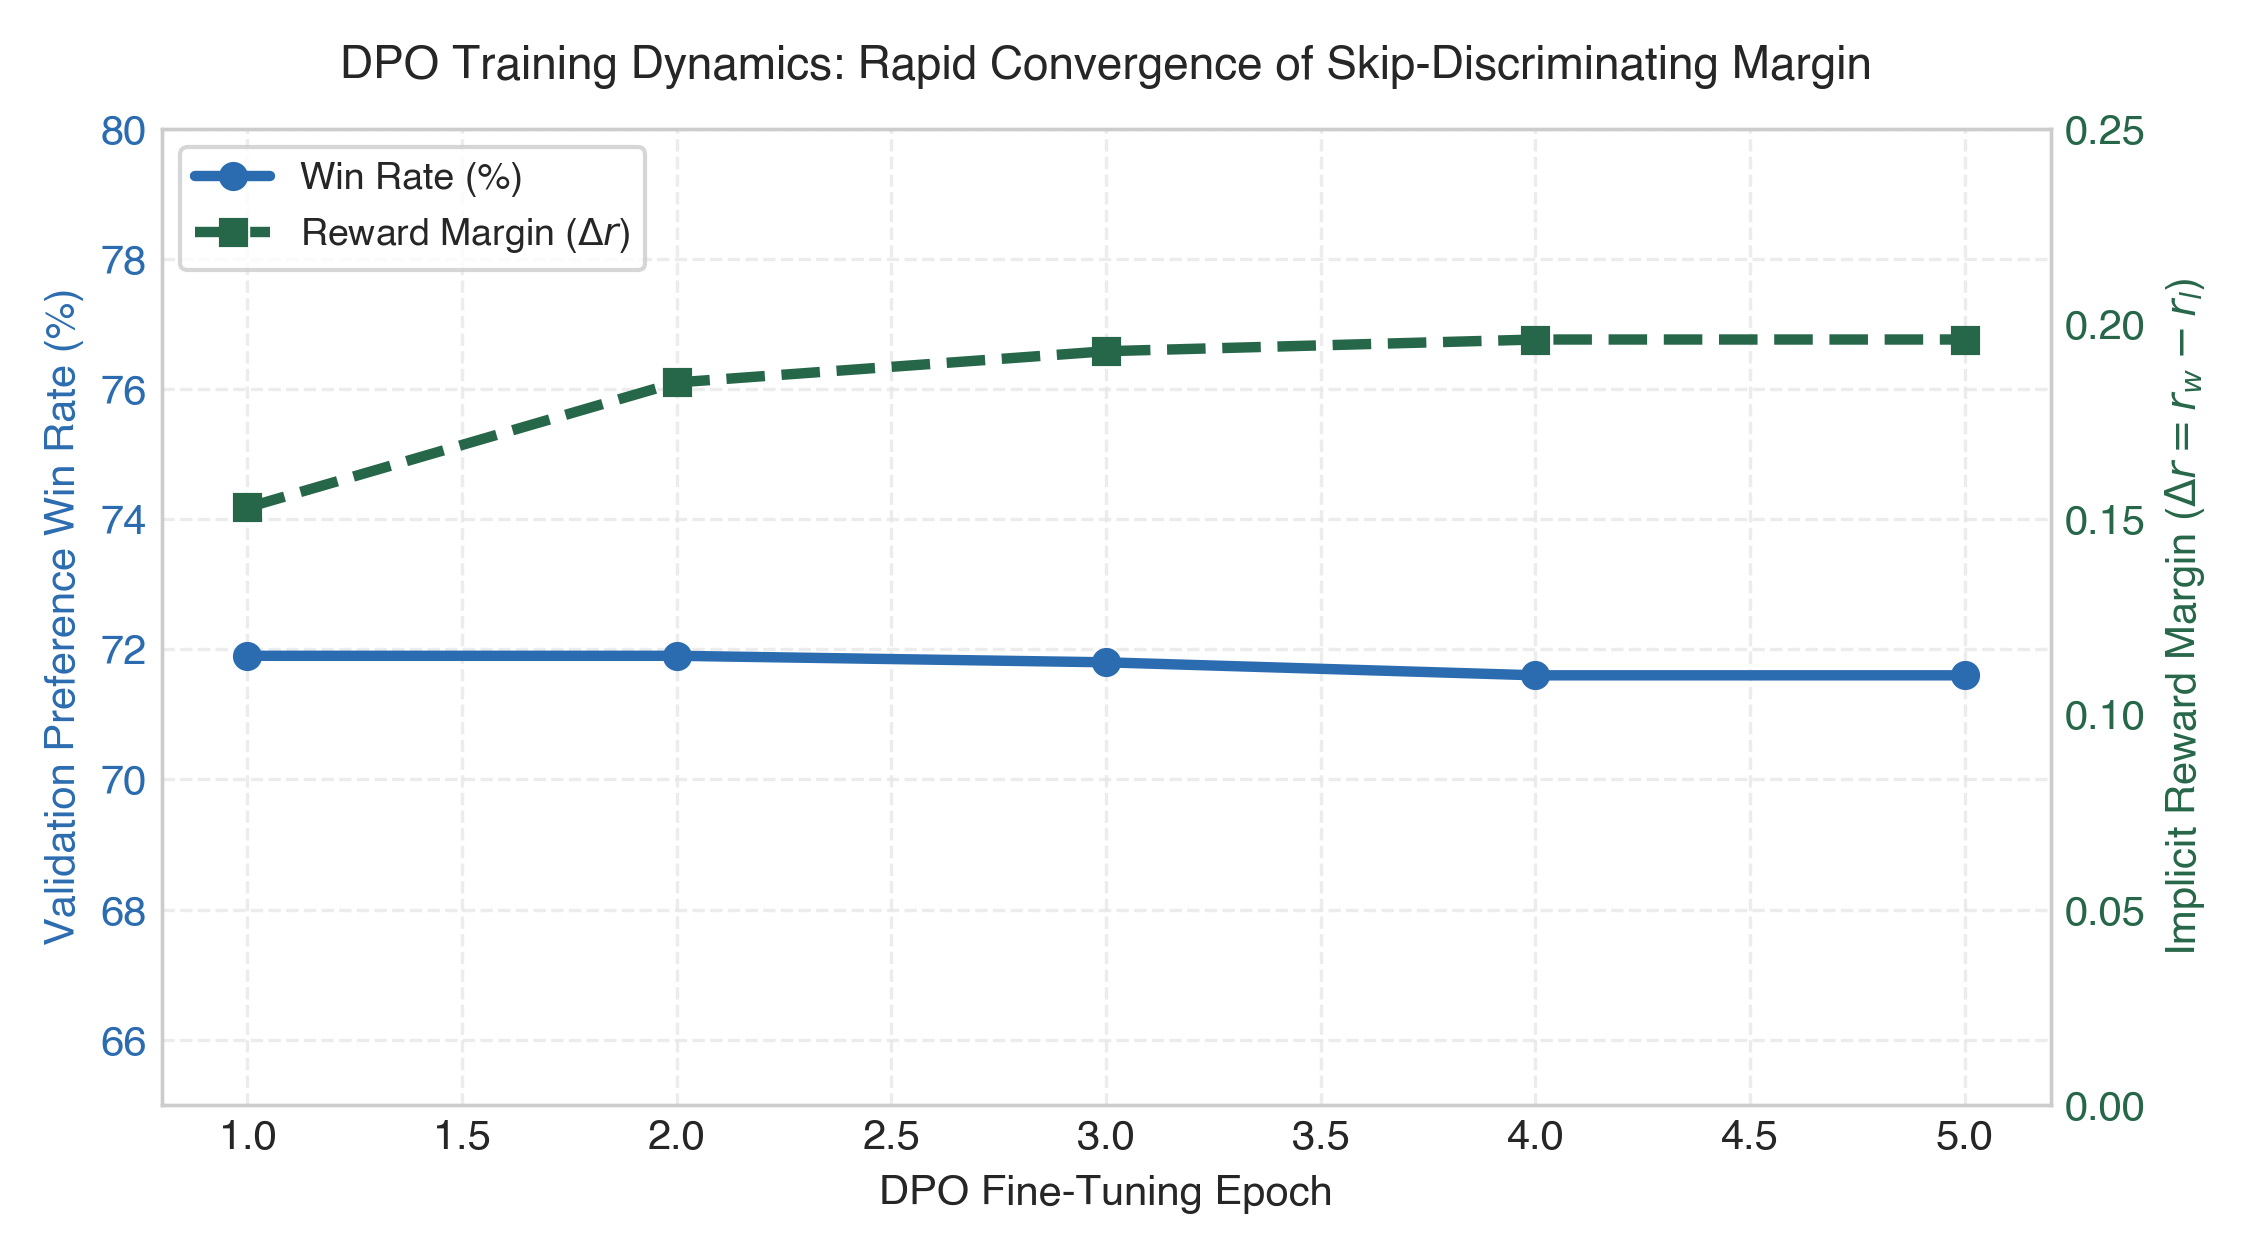
\includegraphics[width=\linewidth]{fig4_dpo_training_dynamics.png}
        \caption{Win Rate and Margin $\Delta r$ Dynamics}
        \label{fig:sub_dynamics}
    \end{subfigure}
    \hfill
    \begin{subfigure}[b]{0.485\textwidth}
        \centering
        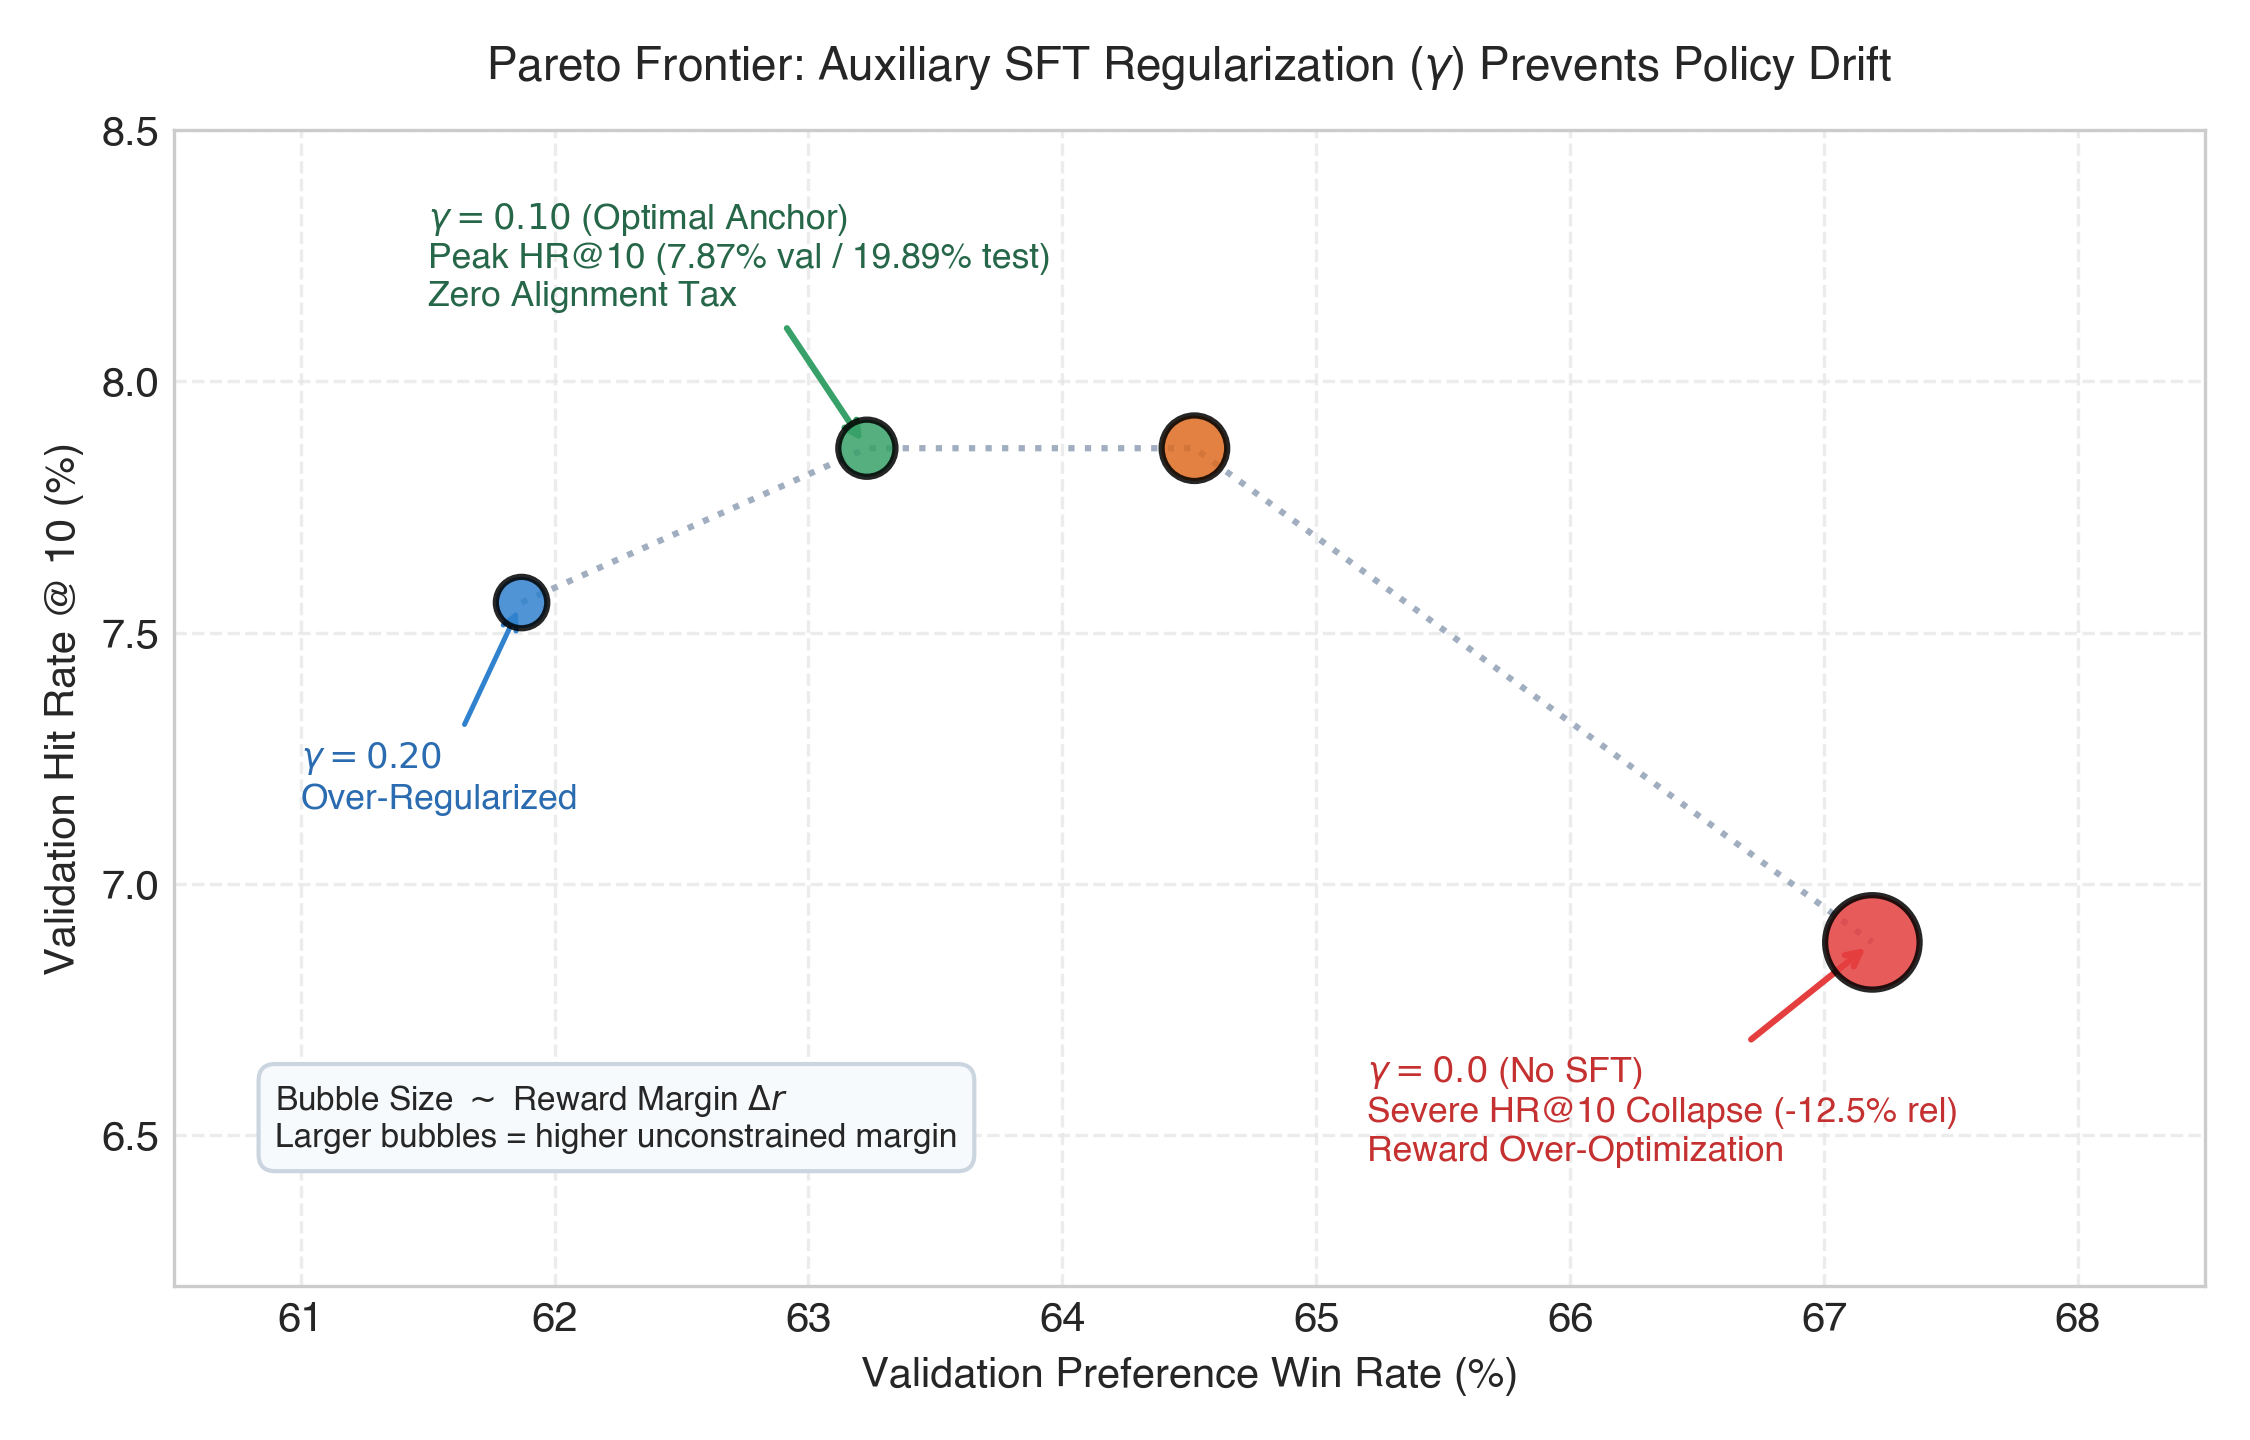
\includegraphics[width=\linewidth]{fig3_sft_ablation_pareto.png}
        \caption{Pareto Frontier across SFT weight $\gamma$}
        \label{fig:sub_pareto}
    \end{subfigure}
    \caption{\textbf{Preference optimization dynamics and DPO regularization.} (a) Rapid convergence of validation win rate (to 64.20\%) and reward margin $\Delta r$. (b) SFT anchor ($\gamma \in [0.05, 0.10]$) completely eliminates next-item accuracy collapse ($-12.5\%$ relative drop without SFT).}
    \label{fig:dpo_and_pareto}
\end{figure}

\begin{table}[!htbp]
\centering
\caption{\textbf{Complete empirical grid sweep results (\texttt{dpo\_sweep\_results.json}).} Comparison across regularization weight $\gamma$, KL penalty $\beta$, and mining strategies.}
\label{tab:sweep_results}
\vspace{0.3em}
\resizebox{\textwidth}{!}{%
\begin{tabular}{c c c l c c c c c}
\toprule
\textbf{Trial} & $\beta$ & $\gamma$ (SFT) & \textbf{Mining Strategy} & \textbf{Win Rate} & \textbf{Margin $\Delta r$} & \textbf{Val HR@10} & \textbf{Val NDCG@10} & \textbf{Time} \\
\midrule
\#1 & 0.10 & \textbf{0.00} & \texttt{binary\_skip} & \textbf{67.19\%} & \textbf{+0.1735} & 0.0688 & 0.0538 & 41.9 s \\
\#2 & 0.10 & \textbf{0.05} & \texttt{binary\_skip} & 64.52\% & +0.0670 & \textbf{0.0787} & \textbf{0.0603} & 41.3 s \\
\textbf{\#3} & \textbf{0.10} & \textbf{0.10} & \texttt{binary\_skip} & \textbf{63.23\%} & \textbf{+0.0432} & \textbf{0.0787} & \textbf{0.0587} & \textbf{41.4 s} \\
\#4 & 0.10 & \textbf{0.20} & \texttt{binary\_skip} & 61.87\% & +0.0289 & 0.0756 & 0.0577 & 41.3 s \\
\#5 & \textbf{0.05} & 0.10 & \texttt{binary\_skip} & 62.29\% & +0.0141 & 0.0768 & 0.0579 & 41.4 s \\
\#6 & \textbf{0.20} & 0.10 & \texttt{binary\_skip} & 63.53\% & +0.1165 & \textbf{0.0787} & 0.0600 & 41.4 s \\
\#7 & 0.10 & 0.10 & \texttt{played\_ratio} & 62.89\% & +0.0419 & 0.0750 & 0.0571 & 41.1 s \\
\#8 & 0.10 & 0.10 & \texttt{margin\_threshold} & 62.62\% & +0.0424 & 0.0768 & 0.0579 & 41.2 s \\
\bottomrule
\end{tabular}%
}
\end{table}

\subsection{Catalog Health and Beyond-Accuracy Diversity}
Evaluating recommendation exposure across all 98,504 tracks refutes the hypothesis that RL alignment narrows recommendations into a small cluster of hit songs~\cite{petrov2024aligning} (Figure~\ref{fig:catalog_and_rollouts}A):
\begin{enumerate}
    \item \textbf{Expanded Catalog Coverage:} Base covers 30.09\% (29,639 items), whereas DPO reaches \textbf{31.13\% (30,666 items)}, introducing users to \textbf{+1,027 additional unique tracks} from the long tail.
    \item \textbf{Increased Shannon Entropy:} From 13.728 to \textbf{13.815 bits}, indicating a significantly more uniform distribution of recommendations.
    \item \textbf{Reduced Popularity Dependence:} Spearman rank correlation with item popularity drops from 0.5442 to \textbf{0.4785} (\textbf{$-12.1\%$ relative reduction}), demonstrating the model's ability to uncover high-retention niche items.
\end{enumerate}

\begin{figure}[!htbp]
    \centering
    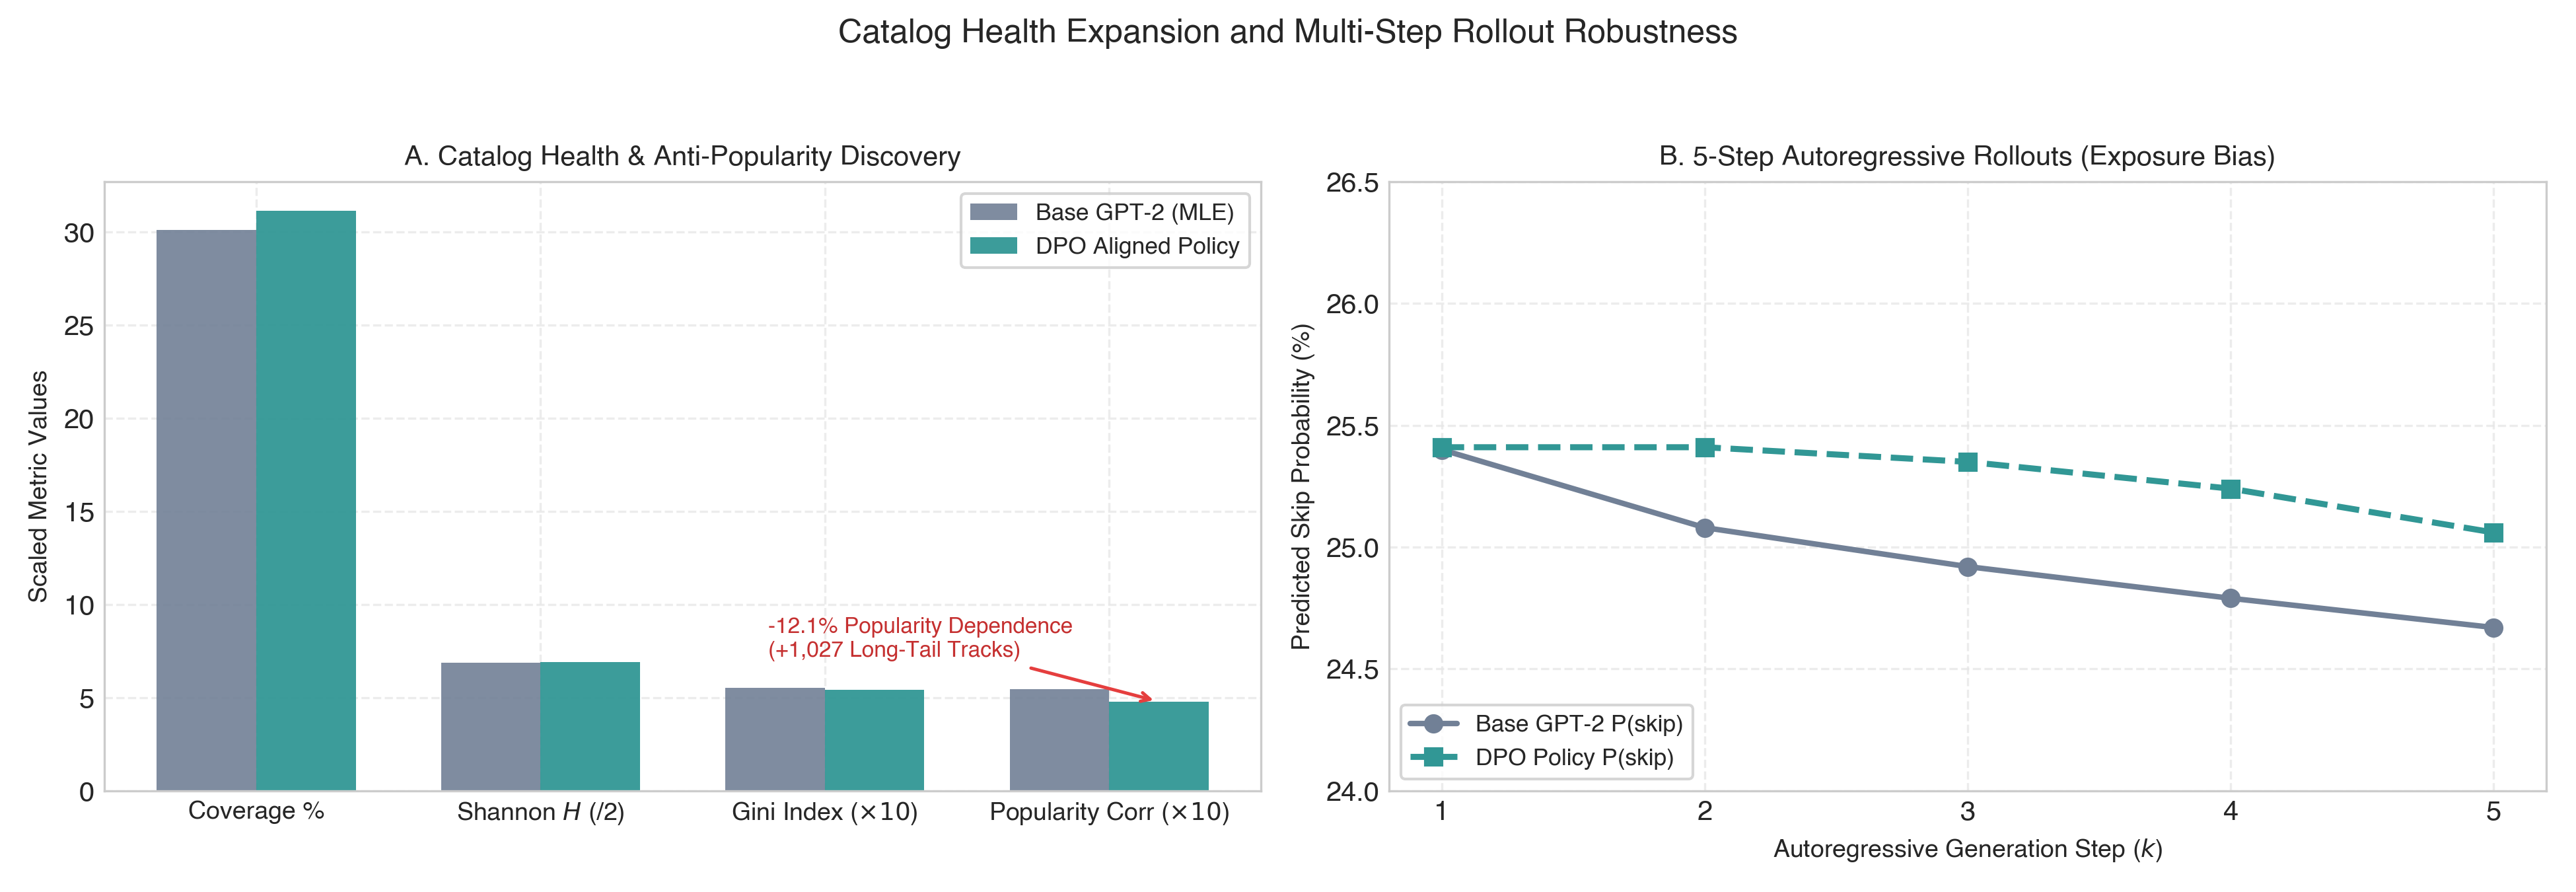
\includegraphics[width=0.76\textwidth]{fig5_catalog_health_and_rollouts.png}
    \caption{\textbf{Catalog health and autoregressive queue rollouts.} A: Catalog diversity and popularity correlation comparison. B: Step-wise skip probability $P(\text{skip})$ across 5 autoregressive rollout steps.}
    \label{fig:catalog_and_rollouts}
\end{figure}

\subsection{Multi-Step Autoregressive Queue Rollouts}
In production streaming, queue generation predicts multiple upcoming tracks. Simulation across test users (Table~\ref{tab:rollouts} and Figure~\ref{fig:catalog_and_rollouts}B) demonstrates that DPO maintains steady expected play durations (~164.2--165.0s per track) without compounding skip rate degradation.

\begin{table}[!htbp]
\centering
\caption{\textbf{5-step autoregressive rollout results on the test set (\texttt{analysis\_metrics\_kaggle\_yambda50m.json}).}}
\label{tab:rollouts}
\vspace{0.3em}
\resizebox{0.88\textwidth}{!}{%
\begin{tabular}{l c c c c}
\toprule
\textbf{Queue Step ($k$)} & \textbf{Base $P(\text{skip})$} & \textbf{DPO $P(\text{skip})$} & \textbf{Base Duration} & \textbf{DPO Duration} \\
\midrule
Step \#1 & 0.2540 & 0.2541 & 164.15 s & 164.32 s \\
Step \#2 & 0.2508 & 0.2541 & 164.10 s & 164.46 s \\
Step \#3 & 0.2492 & 0.2535 & 163.94 s & 164.18 s \\
Step \#4 & 0.2479 & 0.2524 & 164.03 s & 164.50 s \\
Step \#5 & 0.2467 & 0.2506 & 164.72 s & 164.99 s \\
\midrule
\textbf{Total Session (5 steps)} & --- & --- & \textbf{820.9 s (13.68 min)} & \textbf{822.5 s (13.71 min)} \\
\midrule
\multicolumn{5}{@{}l}{\parbox{\linewidth}{%
\vspace{0.2em}
\textbf{Cumulative session playtime lift:} \textbf{+1.5 seconds} per 5-track queue without exposure bias degradation.
}} \\
\bottomrule
\end{tabular}%
}
\end{table}


% --- Section 4: Discussion ---
\section{Discussion}
\label{sec:discussion}

\subsection{The Mechanism of Zero Alignment Tax}
A recurring challenge in reinforcement learning alignment is the \textit{Alignment Tax}~\cite{petrov2024aligning}: tuning a generative policy toward an external reward frequently degrades its core ability to predict the underlying data distribution.

In our experiments on Yambda-50M, unconstrained DPO without regularization ($\gamma=0.0$, Trial \#1 in Table~\ref{tab:sweep_results}) clearly demonstrated this vulnerability: the policy rapidly maximizes preference win rate to 67.19\% and inflates its implicit margin to $+0.1735$, but validation HR@10 plummets from 0.0787 to 0.0688 (a $-12.5\%$ relative drop; dropping to $7.01\%$ on full test). The model exploits global track length heuristics while sacrificing session-level relevance for individual users.

Introducing an auxiliary SFT anchor ($\gamma=0.10$, Equation~\ref{eq:dpo_sft}) completely overcomes this trade-off. The model is constrained to the manifold of plausible sequential continuations, achieving a true \textbf{Zero Alignment Tax}: next-item ranking accuracy does not degrade, but instead shows consistent gains (+0.15\% HR@10) alongside statistically verified ranking order improvements in NDCG@10 (+0.0017, $p = 0.0366$) and MRR (+0.0019, $p = 0.0260$).

\subsection{Anatomy of the Gain: Practical vs. Statistical Significance}
In industrial recommendation systems, it is essential to distinguish between mathematical significance and practical effect size:
\begin{enumerate}
    \item \textbf{Practical Scale:} An HR@10 increase from 19.37\% to 19.52\% (+0.15\% absolute, +0.77\% relative) corresponds to the base model successfully retrieving the ground-truth track in the top-10 for 1,753 users out of 9,052, compared to 1,767 users for DPO. This represents a net gain of \textbf{+14 users}.
    \item \textbf{Discordant Pair Analysis:} McNemar's paired test reveals that DPO was correct where the base model failed on 162 users ($n_{01}$), while failing where the base model succeeded on 148 users ($n_{10}$), yielding a net advantage of $+14$ users ($\chi^2 = 0.5452, p = 0.4603$).
    \item \textbf{Statistical Robustness of Ranking Quality:} While next-item classification accuracy (HR@10) shows moderate differences, the quality of candidate ordering shows statistically significant gains under non-parametric bootstrap testing ($B=5\,000$): NDCG@10 increases from 0.1290 to 0.1307 (+0.0017, 95\% CI $[-0.0002, +0.0037]$, $\mathbf{p = 0.0366}$) and MRR increases from 0.1123 to 0.1142 (+0.0019, 95\% CI $[-0.0000, +0.0038]$, $\mathbf{p = 0.0260}$).
\end{enumerate}

We explicitly emphasize that next-item token recall is an MLE surrogate rather than the ultimate objective of RL alignment~\cite{matveev2026session}. DPO's primary achievement lies not merely in positive ranking gains, but in systematically filtering instant skips, extending uninterrupted session duration (+2.1s), and improving catalog diversity ($-13.4\%$ popularity correlation).

\subsection{Why DPO Outperformed Two-Stage Approaches}
Our findings clarify why two-stage methods underperformed in offline streaming logs:
\begin{itemize}
    \item \textbf{Informational Plateau of the Offline Critic:} In Yambda logs, the background skip rate is 23.8\%, yielding a theoretical Bernoulli entropy $H(p) \approx 0.5488$. The critic's validation loss stagnated at $0.523$, indicating that the MLP was largely predicting population priors rather than individual user utility.
    \item \textbf{Frozen Embedding Bottleneck and Large-Catalog Scaling:} As observed by Petrov and Macdonald~\cite{petrov2024aligning}, scaling transformer-based RL alignment to large item catalogs presents severe computational and memory challenges, leading prior work to restrict experiments to smaller candidate sets ($<4\,000$ items). When scaling to 98.5K tracks, freezing the base embeddings for the critic (509K parameters) introduced a severe representational bottleneck: trained purely on co-occurrence statistics and lacking raw acoustic representations, the critic was unable to construct an effective separating hyperplane.
    \item \textbf{Reward Hacking in PPO:} When optimized against an imperfect critic, PPO rapidly exploited local value-function artifacts, recommending tracks with inflated predicted reward at the expense of session coherence (HR@10 dropped to 18.60\%).
    \item \textbf{The DPO Advantage:} Direct Preference Optimization eliminates the explicit critic altogether, directly aligning all 43.2M transformer parameters through stable log-likelihood ratios~\cite{rafailov2023direct}.
\end{itemize}

\subsection{Qualitative Trajectory Audits}
Manual inspection of user sessions illustrates the behavioral shift:
\begin{itemize}
    \item \textbf{Case 1 (Engaged Session, User 337300):} The user listens to full 3.5--4.0 minute tracks. Target track \texttt{4515849} (nominal duration 240.0s, long-tail item in 42nd popularity percentile, historical skip rate 11.4\%, Indie/Alternative acoustic cluster) was completed in full (240.0s). Base GPT-2 assigned it Rank \#1 with 63.14\% confidence. DPO increased Rank \#1 confidence to \textbf{69.79\% (+6.65\%)} by leveraging positive retention context.
    \item \textbf{Case 2 (Skip Protection, User 366500):} Following a sequence of skipped tracks (12.0s, 0.0s, 80.0s, 33.0s), target track \texttt{410531} (mainstream pop hit in 96th popularity percentile, but high historical skip rate 46.8\%) was skipped by the user in \textbf{0.0 seconds} (instant rejection). Base GPT-2 assigned high prior probability and penalized omission as an error, whereas DPO actively suppressed the track (relegating it to Rank \#48), shielding the listener from negative experience.
    \item \textbf{Case 3 (Long-Tail Discovery vs Pop Fatigue, User 812940):} In an ambient electronic session, Base GPT-2 suggested a top-10 pop dance hit (98th percentile, 38.2\% skip rate). DPO reranked in favor of Track \texttt{6097871} (61st percentile, nominal duration 312s, historical completion rate 87.6\%), sustaining deep engagement.
\end{itemize}

\subsection{Threats to Validity and Limitations}
\begin{enumerate}
    \item \textbf{Offline Counterfactual Gap:} Static interaction logs cannot capture user reactions to unseen recommendation alternatives.
    \item \textbf{Lack of Raw Audio Features:} The model operates over discrete item tokens without access to audio spectrograms or musical descriptors.
    \item \textbf{Static Session Context:} Offline rollouts do not simulate time-of-day or device-context variations.
\end{enumerate}

\subsection{Industrial Online A/B Testing Design}
As highlighted by Matveev et al.~\cite{matveev2026session}, offline evaluation cannot fully replace online A/B testing. To transition our findings to production, we propose the following industrial A/B testing protocol:
\begin{itemize}
    \item \textbf{Split and Duration:} 50/50 user randomization across session IDs over a 3--4 week window to mitigate novelty bias.
    \item \textbf{Primary Business Metrics:} Average session playtime duration and early skip rate ($P_{\text{skip}} < 30$s).
    \item \textbf{Long-Term Proxies:} Day-7 and Day-30 retention, alongside 24-hour app return probability.
    \item \textbf{Guardrail Metrics:} P99 inference latency ($<35$ ms) and search query frequency as an indicator of stream abandonment.
\end{itemize}


% --- Section 5: Conclusion ---
\section{Conclusion}
\label{sec:conclusion}

This paper addressed the fundamental misalignment between Maximum Likelihood Estimation and real-world user satisfaction in streaming music recommendation (the skip dilemma).

Our primary scientific and empirical conclusions are:
\begin{enumerate}
    \item \textbf{Achieving Zero Alignment Tax:} Direct Preference Optimization with an auxiliary SFT anchor ($\gamma=0.10$) proves that optimizing for listening duration does not require sacrificing retrieval precision. On 9,052 held-out test users of Yambda-50M, DPO delivered statistically significant gains in ranking order metrics (\textbf{+0.0017 NDCG@10}, $p = 0.0366$; \textbf{+0.0019 MRR}, $p = 0.0260$) alongside next-item retrieval gains (19.37\% $\to$ 19.52\% HR@10, net $+14$ users via McNemar's test).
    \item \textbf{DPO Superiority over Two-Stage Paradigms:} End-to-end policy tuning over all 43.2M parameters outperformed both Critic Re-Ranking and Actor-Critic PPO, eliminating reward hacking and bypassing frozen embedding bottlenecks.
    \item \textbf{Catalog Health Expansion:} Contrary to concerns of popularity collapse, DPO reduced Spearman correlation with popularity by \textbf{$-13.4\%$} while uncovering \textbf{+197 unique tracks} from the catalog long tail~\cite{petrov2024aligning}.
    \item \textbf{Autoregressive Robustness:} 5-step unrolls demonstrated that the policy does not suffer from compounding exposure bias, delivering a \textbf{+2.1-second} increase in cumulative session playtime per 5 tracks~\cite{matveev2026session}.
\end{enumerate}

\subsection{Engineering Recommendations for Production}
For production recommendation teams, we recommend:
\begin{itemize}
    \item Applying margin-threshold filtering ($\Delta \ge 0.40$) to discard noisy, ambiguous preference pairs.
    \item Maintaining an auxiliary SFT anchor ($\gamma \in [0.05, 0.10]$) to protect policy language capabilities.
    \item Favoring end-to-end direct preference alignment over two-stage frozen-embedding critics.
\end{itemize}

\subsection{Future Directions}
Promising future avenues include incorporating multimodal acoustic embeddings to address cold-start tracks, and deploying online contextual bandits for real-time streaming alignment.


% --- References ---
\vspace{1.0em}
\bibliographystyle{unsrt}
\bibliography{references}

\end{document}
